% CREATED BY DAVID FRISK, 2016
\chapter{Results and discussion}
% Describe you results. Use tables, diagrams etc. for illustration.

\section{Performance}

% Undersök varför inte alla meningar ger samma resultat
% Kör hela upto12eng och jämför diff för statistik och hitta mönster

% Idé: Scatter-plot av optimerad mot ooptimerad

The result of running different versions of the algorithm on the example file called \texttt{upto12eng.conllu} using the example grammar \texttt{ShallowParse} in the gf-ud git repository can be seen in \autoref{fig:time-including-gc}. The full list of sentences included in the benchmark can be seen in \autoref{app:upto12}. All benchmarks were perfomed on a 2019 MacBook Pro, with a 2.3 GHz 8-Core Intel Core i9 CPU.

\begin{table}[]
    \centering
    \begin{tabular}{c|ccc}
    Time (seconds) & Calculation & Garbage Collection & Total \\
    \hline
    Original code & 2m 58.8s & 24.6s & 3m 23.5s \\
    Original code (fast GC) & 3m 01.9s & 20.2s & 3m 22.1s \\
    fastKeepTrying & 26.2s & 14.7s & 40.9s \\
    fastKeepTrying (fast GC) & 28.6s & 1.7s & 30.3s \\
    fastAllFunsLocal & 3.2s & 14.3s & 17.2s \\
    fastAllFunsLocal (fast GC) & 3.2s & 1.3s & 4.5s \\
    Both improvements & 2.7s & 13.9s & 16.6s \\
    Both improvements (fast GC) & 1.25s & 1.25s & 2.5s \\
    \end{tabular}
    \caption{The total run time for converting the file upto12eng.conllu, including garbage collection and startup time. The bars marked ``fast GC'' have increased initial heap size to 500Mb to reduce the number of unnecessary garbage collections, based on the experiments in \autoref{sect:gc-time}. Each measurement was only performed once, so there might be some inaccuracy because of random noise resulting from preemptive multitasking. }
    \label{tab:time-with-gc}
\end{table}

In \autoref{fig:time-vs-time} we can see the speedup for each individual sentence. The improvement of the keepTrying function gives a close to linear speedup, while the speedup from the optimized version of allFunsLocal is much larger. The theoretical expected speedup from keepTrying is a quadratic factor that becomes a linear factor based on the depth of the resulting trees. The library Criterion\protect\footnotemark{} was used to perform the measurements. A full table of results can be found in \autoref{appendix:performance}.
\begin{figure}
    \centering
    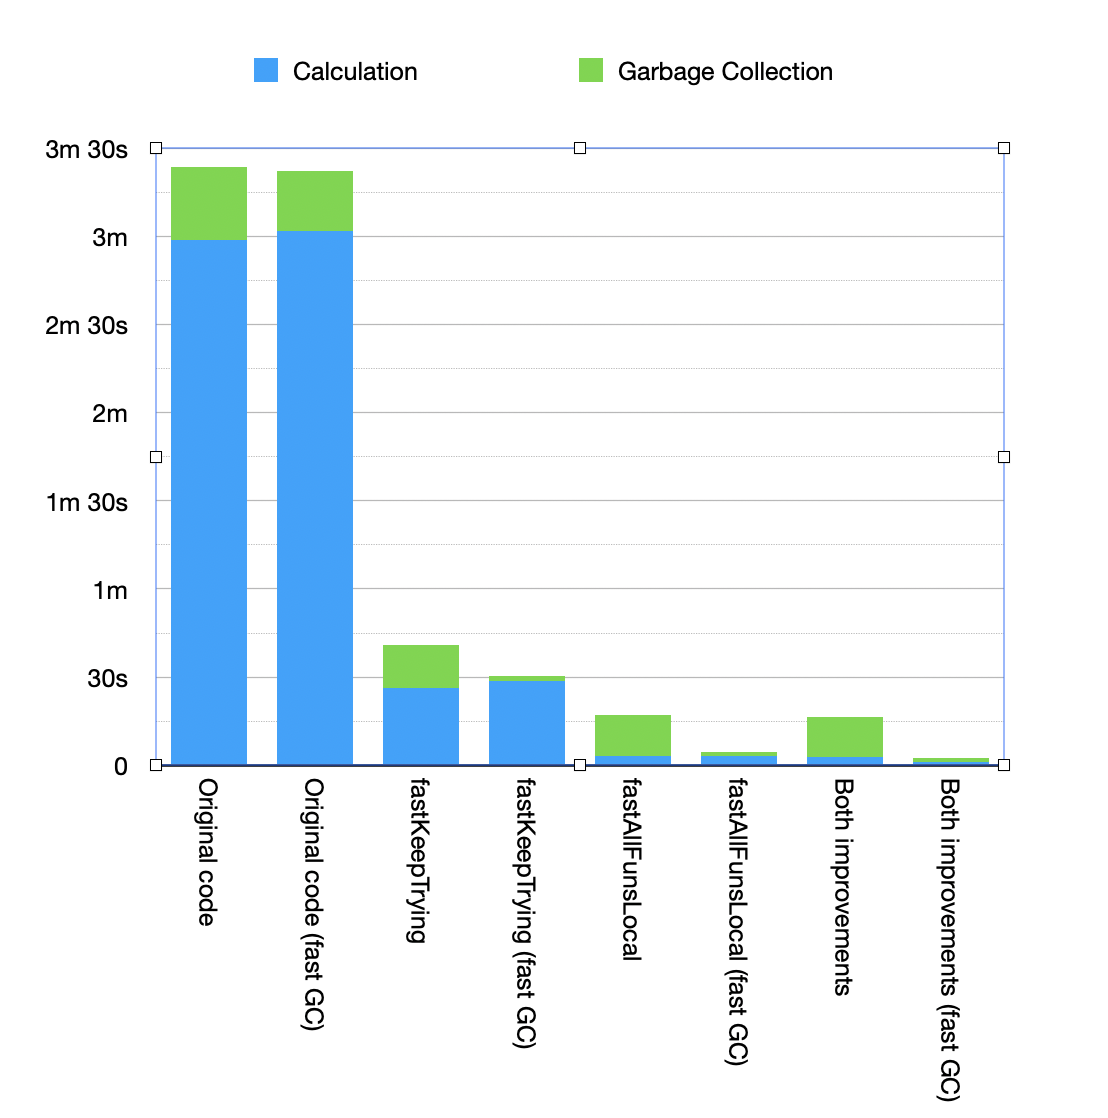
\includegraphics[scale=0.75]{figure/Time-including-GC.png}
    \caption[The total run time for converting the file \texttt{upto12eng.conllu}, including garbage collection and startup time.]{The total run time for converting the file \texttt{upto12eng.conllu}, including garbage collection and startup time. The bars marked ``fast GC'' have increased initial heap size to 500Mb to reduce the number of unnecessary garbage collections, based on the experiments in \autoref{sect:gc-time}. Each measurement was only performed once, so there might be some inaccuracy because of random noise resulting from preemptive multitasking.}
    \label{fig:time-including-gc}
\end{figure}
\begin{figure}
    \centering
    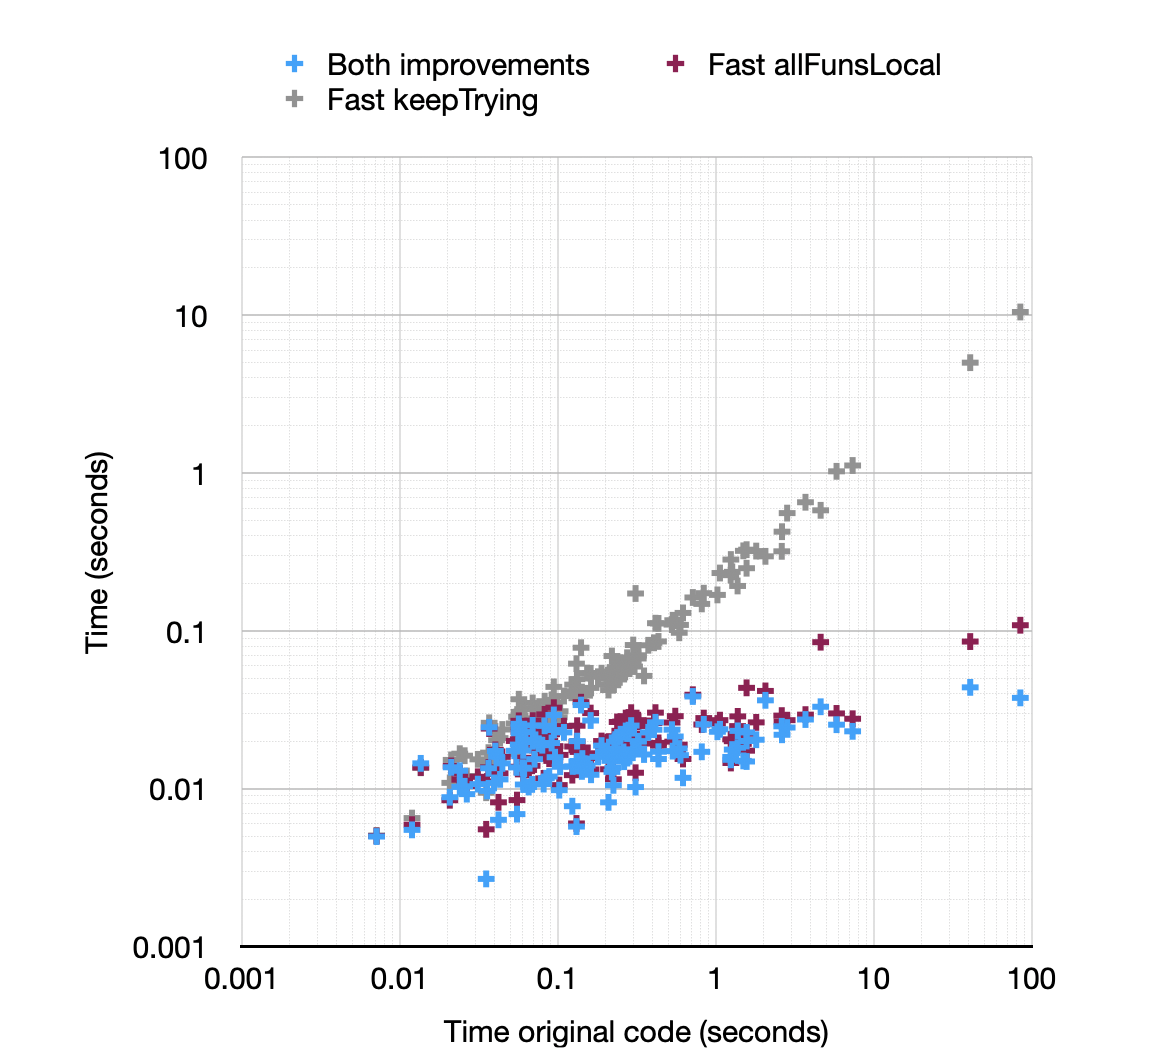
\includegraphics[scale=0.7]{figure/Time-against-time-plot.png}
    \caption{A log-log plot of time for each optimization against the time for the original algorithm. Each data point is the average time over several runs for a single sentence. The library Criterion\protect\footnotemark{} was used to perform the measurements.}
    \label{fig:time-vs-time}
\end{figure}
\footnotetext{http://www.serpentine.com/criterion/}
 
In \autoref{fig:keepTrying-speedup-factor} we can see that the speedup from the keepTrying improvement is linear with respect to the logarithm of the original code, which matches the expectation of moving from converting a quadratic factor to a linear factor. 
Looking at the slowest sentence ``In Danish, the word may even apply to shallow lagoons'', it takes 83 seconds with the original algorithm and 10 seconds with the keepTrying improvement, giving a speedup factor of 8.3. Looking at the generated tree we can confirm that it has a maximum tree depth of 9 at the top, matching the expectation.

\begin{figure}
    \centering
    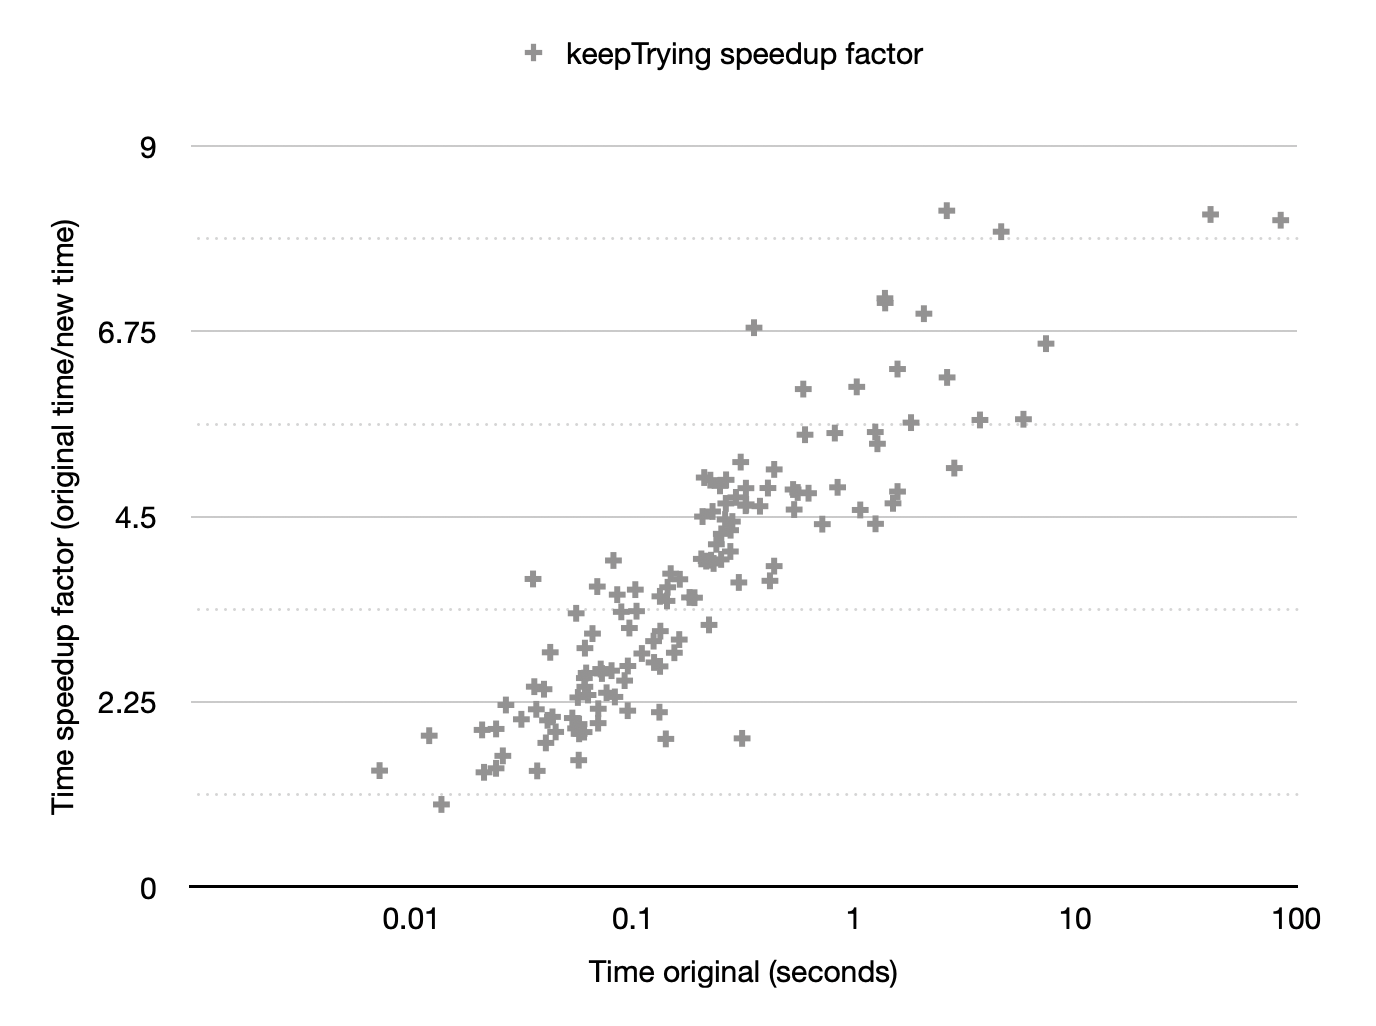
\includegraphics[scale=0.5]{figure/keepTrying-speedup-factor.png}
    \caption{A plot of the speedup factor for the improved keepTrying algorithm: new time divided by original time, against the original time taken. A linear speedup is the expected result for converting a quadratic algorithm to a linear algorithm.}
    \label{fig:keepTrying-speedup-factor}
\end{figure}

In \autoref{fig:allFunsLocal-speedup-factor} we can see that the allFunsLocal improvement has a speedup factor that is linear on the log-log plot, which indicates that we got an exponential speedup as expected from the theory.

\begin{figure}
    \centering
    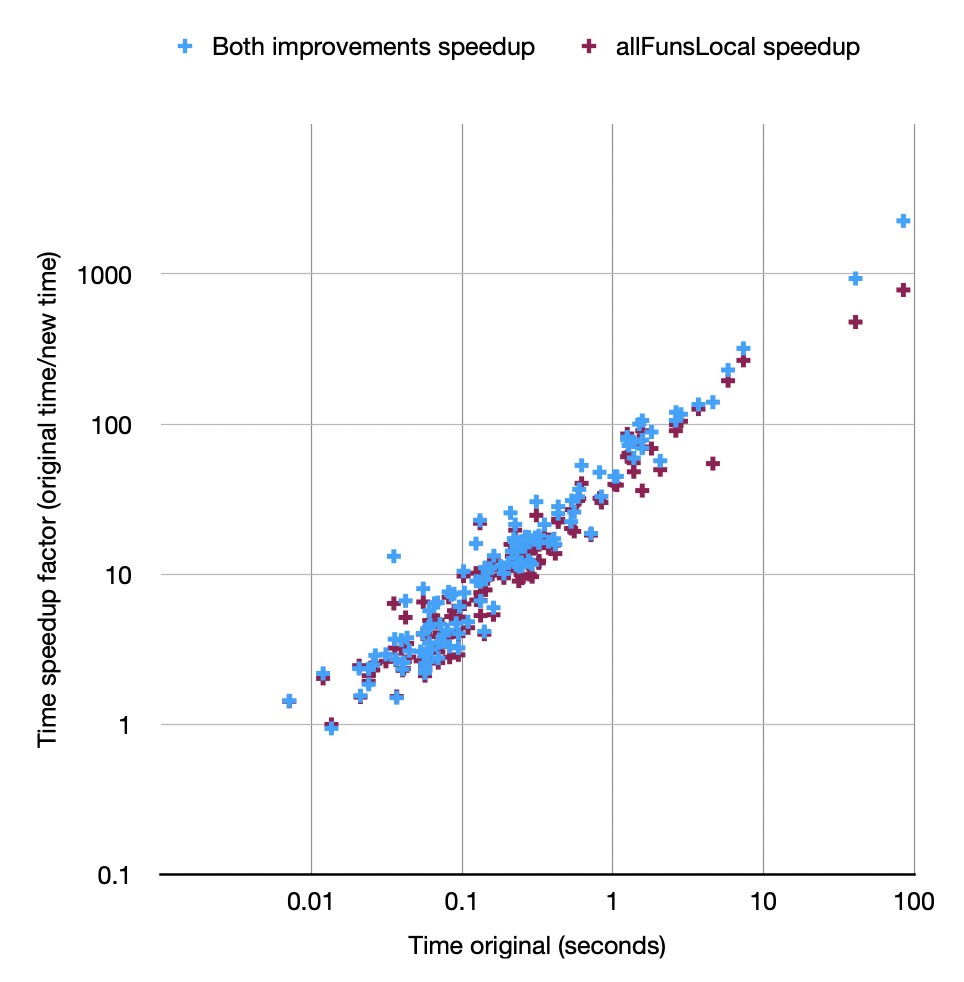
\includegraphics[scale=0.75]{figure/allFunsLocal-speedup-factor.png}
    \caption{A log-log plot of the speedup factor for the improved allFunsLocal algorithm: new time divided by original time, against the original time taken. The linear pattern indicates an exponential speedup.}
    \label{fig:allFunsLocal-speedup-factor}
\end{figure}

% DONE: Write about the minor changes in the resulting trees from the optimized version of the keepTrying function.

% DONE: \todo[inline]{Stacked diagram of all four configurations, with GC time included}


% Running on upto12eng with both improvements and default Garbage Collection settings
% \begin{verbatim}
%    7,783,705,112 bytes allocated in the heap
%   13,905,705,592 bytes copied during GC
%      178,448,096 bytes maximum residency (37 sample(s))
%        2,051,952 bytes maximum slop
%              516 MiB total memory in use (0 MB lost due to fragmentation)
% 
%                                      Tot time (elapsed)  Avg pause  Max pause
%   Gen  0      7351 colls,     0 par    9.128s   9.260s     0.0013s    0.0056s
%   Gen  1        37 colls,     0 par    4.828s   5.069s     0.1370s    0.2165s
% 
%   INIT    time    0.000s  (  0.005s elapsed)
%   MUT     time    2.612s  (  2.666s elapsed)
%   GC      time   13.956s  ( 14.329s elapsed)
%   EXIT    time    0.000s  (  0.005s elapsed)
%   Total   time   16.569s  ( 17.004s elapsed)
% 
%   %GC     time       0.0%  (0.0% elapsed)
% 
%   Alloc rate    2,979,803,301 bytes per MUT second
% 
%   Productivity  15.8% of total user, 15.7% of total elapsed
% \end{verbatim}


\subsection{Garbage Collection time}\label{sect:gc-time}
As we saw in \autoref{fig:time-including-gc} and \autoref{tab:time-with-gc}, when the optimized algorithm is used, over 80\% of time is spent on garbage collection. This is in a large part because GHC uses a generational, moving garbage collector\cite{ungar1984generation}, which means that the cost of a garbage collection is proportional to the amount of currently living data. % \todo{Source for this claim}
In our case we have a large amount of long-living data, which means that every major garbage collection is expensive. The code begins by loading the GF grammar into memory, which for our test grammar takes up around 100 megabytes. There are several ways to mitigate this, but the easiest solution is to tweak the parameters for the garbage collector to make it wait longer before attempting to collect garbage, which reduces the total number of major garbage collections.
% Nope: \todo[inline]{The text above should probably go elsewhere (if anywhere at all)}

The tool ghc-gc-tool allows automatically determining which parameters are best for this by running the executable with different parameters and plotting the result. In \autoref{fig:gf-ud-integ-gc-space} we can see the result of running this on the first 60 items of upto12eng.conllu with the ShallowParse grammar from the repository. This number was chosen arbitrarily to make the runtime not be unreasonably long. 

As can be seen in \autoref{fig:GC-time} any initial heap size over 256M drastically reduces the run time and the logs show that the productivity (time spent on non-GC) goes from 15\% to 50\% and that less than one tenth as many garbage collections are performed. This number depends on the size of the GF grammar and it corresponds to the size of the GF grammar after being loaded into memory. Running the command with the default GC parameters shows that the maximum residency is 180M, which is slightly less than the optimal GC parameter value.

\begin{verbatim}
$ ghc-gc-tune -t pdf -spr gf-ud ud2gf grammars/ShallowParse Eng Text
...
gf-ud +RTS -A32768 -H134217728 -RTS ud2gf grammars/ShallowParse Eng Text
    <<GCs 125563, peak   538, resident 177.67m, MUT 1.728s, GC 9.609s>>
gf-ud +RTS -A32768 -H268435456 -RTS ud2gf grammars/ShallowParse Eng Text
    <<GCs   8655, peak   509, resident 176.64m, MUT 1.211s, GC 1.776s>>
...
\end{verbatim}

\begin{figure}
    \centering
    \subcaptionbox{Integral of space use over time\label{fig:GC-time-integ}}
      {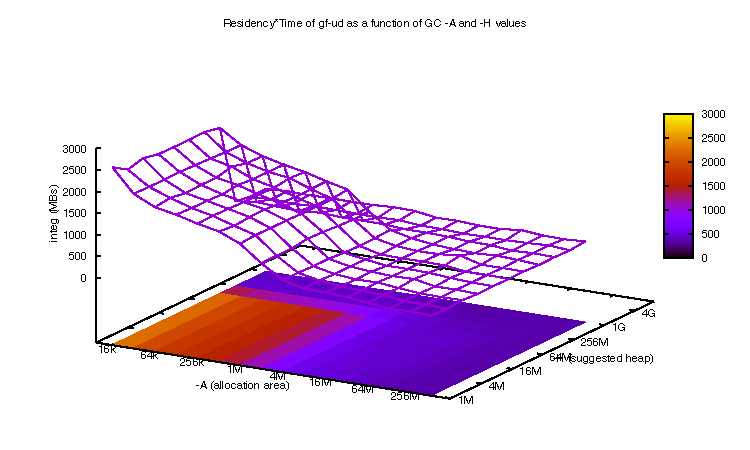
\includegraphics[scale=0.5]{figure/gf-ud-integ-gc-space.pdf}}
    \subcaptionbox{Time taken\label{fig:GC-time}}
      {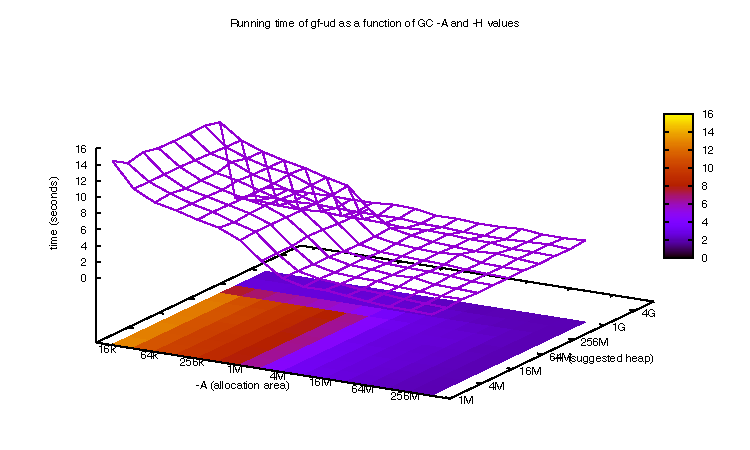
\includegraphics[scale=0.5]{figure/gf-ud-time-gc-space.pdf}}
    \subcaptionbox{Resident space usage\label{fig:GC-resident-space}}
      {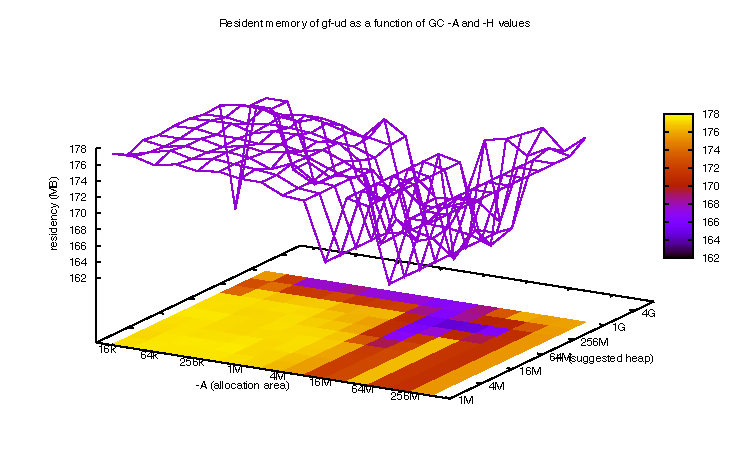
\includegraphics[scale=0.5]{figure/gf-ud-residency-gc-space.pdf}}
    \subcaptionbox{Peak space usage\label{fig:GC-peak-space}}
      {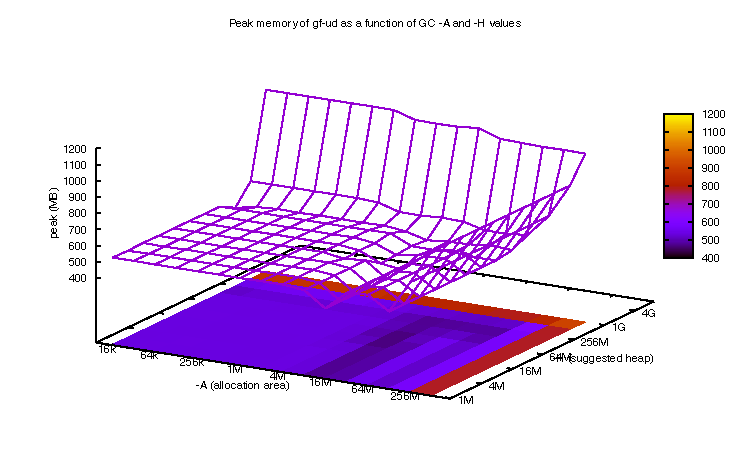
\includegraphics[scale=0.5]{figure/gf-ud-peak-gc-space.pdf}}
    \caption{The integral of space usage over time for different GC parameters}
    \label{fig:gf-ud-integ-gc-space}
\end{figure}

We also explored other methods for reducing the impact of garbage collection, like compact regions\cite{yang2015efficient}, but they provided no improvement over the simpler method of tweaking the GC parameters and in some cases using them made performance worse, because they force all data stored to be fully evaluated.

\section{Correctness}

Because the accuracy of the conversion depends on manually written annotation files, evaluating the accuracy of the conversion is outside of the scope for this paper.

The optimization of the \texttt{allFunsLocal} function had no impact on the generated trees. However, in some cases the optimization of the \texttt{keepTrying} functions caused different trees to be picked. The different trees are equally valid according to the defined constraints in the annotations and some of them are better and some are worse fits in the example trees we evaluated. See \autoref{sec:multiple_trees} for more details on the multiple possible trees.

\section{Debugging}

The debugging tool that was written in this project allows finding what prevented an \#auxfun macro from being used to convert a tree and anecdotal evidence points towards it being helpful when writing annotations.


\section{Flexibility}

%The new recursive macros made it possible to express the tree shape changes required to convert from the UD way of writing coordination into the GF way of writing conjunctions. Initial tests were successful in converting coordinate structures\footnote{For example ``furry, fluffy and cute'' or ``dog, cat or capybara''} of different lengths and different parts of speech. 

The new recursive macros made it possible to express more significant changes in tree shapes when converting between UD and GF. The motivating example is \emph{coordination}: structures like ``big \emph{or} small'' or ``cats, dogs \emph{and} capybaras''. Before the recursive macros, it was only possible to convert structures with exactly 2 conjuncts, since those had sufficiently similar structure, but now ud2gf can convert coordinate structures of arbitrary length.


\section{Use in robust parsing}

As mentioned in \autoref{sect:background}, the improvement of ud2gf was done as a part of the SMU CCLAW project, with the goal of using ud2gf as a part of a pipeline for parsing unrestricted text in the legal domain.
Experiments on that were performed on a small scale, but the results were deemed unsatisfactory for that specific use. A major part of the problem was the correctness of udpipe itself: legal text contains many uncommon structures, and the initial parses were inaccurate relatively often. 
Given the dissatisfaction with the approach, we never did a quantitative evaluation of the results.

Anecdotally, we found the macro system useful in recovering from parser errors, but it was a lot of tedious work\footnote{Example auxfuns written to recover from errors in udpipe output can be found at \url{https://github.com/smucclaw/sandbox/blob/default/inari/ud/copied-from-dsl/grammars/UDAppEng.labels\#L105-L136}}, with a long tail of fixes that only applied to a single sentence. 

% Write something about the results of using it in the singapore project

% Tie back to section 1.4

% Notes:
% Move info about the singapore project earilier in intro
%

